\documentclass[a4paper, 12pt]{article}
\usepackage[a4paper,top=1.5cm, bottom=1.5cm, left=1cm, right=1cm]{geometry}

% Работа с русским языком
\usepackage[utf8]{inputenc}
\usepackage{mathtext}                % русские буквы в формулах
\usepackage[english, russian]{babel} % локализация и переносы

\usepackage{graphicx}   % Вставка изображений
\usepackage{float}      % "Плавающие" изображения3
\usepackage{wrapfig}    % Обтекание фигур (таблиц, картинок и прочего)
\graphicspath{ {./images/} }

\usepackage{tabularx}
\usepackage{multirow}
\usepackage{amsmath}
\usepackage{amsfonts}
\usepackage{indentfirst}
\usepackage{longtable}
\graphicspath{{pictures/}}
\usepackage{natbib}

%%% Колонтитулы
\usepackage{titleps}
\newpagestyle{main}{
	\setheadrule{0.4pt}
	\sethead{Свободные и вынужденные колебания в электрическом контуре}{}{}
	\setfootrule{0.4pt}                       
	\setfoot{ФРКТ МФТИ, 2023}{}{\thepage} 
}
\pagestyle{main}  

\begin{document}
    \begin{titlepage}
	\begin{center}
            {\large МОСКОВСКИЙ ФИЗИКО-ТЕХНИЧЕСКИЙ ИНСТИТУТ (НАЦИОНАЛЬНЫЙ ИССЛЕДОВАТЕЛЬСКИЙ УНИВЕРСИТЕТ)}
	\end{center}
 
	\begin{center}
		{\large Физтех-школа радиотехники и компьютерных технологий}
	\end{center}
	
	\vspace{8cm}
	{\LARGE
		\begin{center}
                {\bf Отчёт о выполнении лабораторной работы 3.2.5}\\
                Свободные и вынужденные колебания в электрическом контуре
		\end{center}
	}
	\vspace{5cm}
	\begin{flushright}
		{\Large Автор:\\ Тихонов Дмитрий Романович, \\
			\vspace{0.2cm}
			студент группы Б01-206}
	\end{flushright}
	\vspace{5cm}
	\begin{center}
		\Large Долгопрудный, 2023
	\end{center}
    \end{titlepage}

    \section{Введение}

    \par \textbf{Цель работы:} исследование свободных и вынужденных колебаний в колебательном контуре. \\

    \par \textbf{В работе используются:} осциллограф АКТAКОM ADS-6142H, генератор сигналов специальной формы АКИП-3409/4, магазин сопротивления МСР-60, магазин емкости Р5025, магазин индуктивности Р567 типа МИСП, соединительная коробка с шунтирующей емкостью, соединительные одножильные и коаксиальные провода.
    
    \section{Теоретические сведения}

    \subsection{Свободные колебания}

    Рассмотрим электрический контур, состоящий из последовательно соединённых конденсатора $С$, резистора $R$ и катушки индуктивности $L$ (рис. \ref{circuit1}).

    \begin{figure}[H]
        \centering
        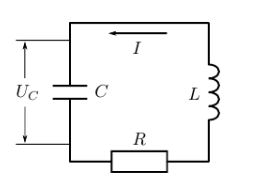
\includegraphics{images/circuit_1.png}
        \caption{Последовательный колебательный контур}
        \label{circuit1}
    \end{figure}

    Сумма падений напряжения на элементах цепи в отсутствие внешней ЭДС равна нулю:

    \begin{equation}
        RI + U_C + L \frac{dI}{dt} = 0
        \label{diffur_eds_01}
    \end{equation}

    Подставив в уравнение (\ref{diffur_eds_01}) выражение для $I = \frac{dq}{dt} = C \frac{dU_C}{dt}$, получим:

    \begin{equation}
        CL \frac{d^2U_C}{dt^2} + CR \frac{dU_C}{dt} + U_C = 0
    \end{equation}

    Разделим это уравнение на $CL$ и введём обозначения

    \begin{equation}
        \gamma = \frac{R}{2L}, \: {\omega_0}^2 = \frac{1}{LC},
        \label{definition_1}
    \end{equation}

    где $\gamma$ -- \textit{коэффициент затухания}, $\omega_0$ -- \textit{собственная круговая частота колебательного контура}. В итоге получим:

    \begin{equation}
        \Ddot{U}_C + 2\gamma \Dot{U}_C + \omega_0^2 U_C = 0
        \label{diffur_eds_02}
    \end{equation}

    Для решения уравнения (\ref{diffur_eds_02}) введём вспомогательную переменную $U_C(t) = U(t) e^{-\gamma t}$:

    \begin{equation}
        \Ddot{U} + \omega_1^2 U = 0,
        \label{diffur_main_1}
    \end{equation}

    где 

    \begin{equation}
        \omega_1^2 = \omega_0^2 - \gamma^2
        \label{omega_1}
    \end{equation}

    В зависимости от соотношения между коэффициентом затухания $\gamma$ и собственной частотой $\omega_0$ возможны затухающие колебания ($0 < \gamma < \omega_0$), критический режим ($\gamma = \omega_0$) и апериодический режим ($\gamma > \omega_0$). Будем рассматривать первый случай, тогда можно записать:

    \begin{equation}
        0 < R < 2 \sqrt{\frac{L}{C}} = R_{cr}, \: \rho = \frac{1}{2} R_{cr},
    \end{equation}

    где $R_{cr}$ -- \textit{критическое сопротивление}, $\rho$ -- \textit{волновое сопротивление}.

    Можно записать решение исходного уравнения (\ref{diffur_main_1}) в виде

    \begin{equation}
        U_C(t) = U_0 e^{-\gamma t} \cos(\omega_1 t + \varphi_0) = e^{-\gamma t} (a \cos{\omega_1 t} + b \sin{\omega_1 t})
        \label{ans_diffur_1}
    \end{equation}

    Из начальных условий можно получить:

    \begin{equation}
        \tg{\varphi_0} = -\gamma/\omega_1, \: I_0 = \frac{U_0}{\rho}
        \label{start_cond}
    \end{equation}

    Из (\ref{start_cond}) видно, что волновое сопротивление контура $\rho$ есть отношение \textit{<<амплитуд>>} затухающих колебаний напряжения на конденсаторе и тока в контуре.

    Выразив $a$ и $b$ из уравнения (\ref{ans_diffur_1}), можно получить:

    \begin{equation}
        U_C(t) = U_{C0} e^{-\gamma t} \left( \cos{\omega_1 t} + \frac{\gamma}{\omega_1} \sin{\omega_1 t} \right), \: I(t) = C\Dot{U}_C
        \label{phase}
    \end{equation}

    Из формул (\ref{phase}) следует параметрическое представление траектории системы на фазовой плоскости переменных $(U_C, I)$. Задание этих двух величин полностью определяет состояние системы в момент времени $t$. 
    
    На рис. \ref{fig:phase}а показаны в безразмерных переменных зависимости (\ref{phase}) напряжения и тока в контуре от времени в режиме свободных затухающих колебаний. На рис. \ref{fig:phase}б показана фазовая траектория этих колебаний на плоскости переменных $(u, j)$, представляющая собой скручивающуюся к точке $(0, 0)$ спираль.

    \begin{figure}[H]
        \centering
        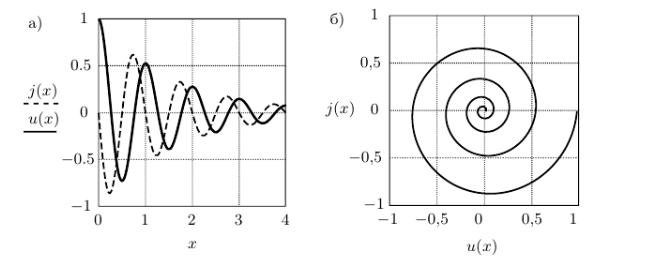
\includegraphics{images/phase.png}
        \caption{Затухающие колебания при $\gamma/\omega_0 =0.1 $: а) ток в контуре $j(x)$ и напряжение на конденсаторе $u(x)$, б) траектория системы на фазовой плоскости $j(u)$}
        \label{fig:phase}
    \end{figure}

    В качестве характеристик процесса затухания колебаний помимо коэффициента затухания $\gamma$ используют \textit{время затухания}:

    \begin{equation}
        \tau = \frac{1}{\gamma} = \frac{2L}{R},
        \label{tau}
    \end{equation}

    то есть время, за которое амплитуда колебаний убывает в $e$ раз, а также \textit{логарифмический декремент}, который равен обратному числу $N_\tau$ периодов $T_1 = \frac{2 \pi}{\omega_1}$, за которое амплитуда колебаний уменьшается в $e$ раз:

    \begin{equation}
        \Theta = \ln{\frac{U_k}{U_{k+1}}} = \frac{1}{n}  \ln{\frac{U_k}{U_{k+n}}} = \gamma T_1 = \frac{1}{N_\tau}
    \end{equation}

    С логарифмическим декрементом связана ещё одна характеристика колебательного контура — его \textit{добротность} $Q$:

    \begin{equation}
        Q \equiv \frac{\pi}{\Theta} = \frac{\pi}{\gamma T_1} = \frac{1}{2} \sqrt{\frac{\omega_0^2}{\gamma^2} - 1} = \frac{1}{2} \sqrt{\frac{R_{cr}^2}{R^2} - 1} = \sqrt{\frac{\rho^2}{R^2} - \frac{1}{4}}
    \end{equation}

    Рассмотрим колебательный контур со \textit{слабым} затуханием, то есть такой, что $Q \gg 1$, тогда $0 < \gamma \ll \omega_0$. Отсюда,

    \begin{equation}
        Q \approx \frac{\pi}{\gamma T_0} = \frac{\tau \omega_0}{2} = \frac{1}{R}\sqrt{\frac{L}{C}} = \frac{\rho}{R}
        \label{approxQ}
    \end{equation}

    \subsection{Вынужденные колебания}
    
    Рассмотрим процессы, протекающие в контуре, подключённом к источнику внешней ЭДС, изменяющейся по гармоническому закону $\mathcal{E} = \mathcal{E}_0 \cos(\omega t + \varphi_0)$. Соответствующая схема представлена на рис. \ref{circuit2}.

    \begin{figure}[H]
        \centering
        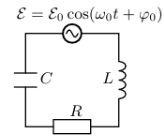
\includegraphics{images/circuit2.png}
        \caption{Последовательный контур с внешней ЭДС}
        \label{circuit2}
    \end{figure}

    Для напряжения на конденсаторе $U_C(t)$ вместо (\ref{diffur_eds_02}) получим теперь уравнение

    \begin{equation}
        \Ddot{U}_C + 2 \gamma \Dot{U}_C + \omega_0^2 U_C = \omega_0^2 \mathcal{E}_0 \cos(\omega t + \varphi_0)
        \label{forced_fluctuations_1}
    \end{equation}

    Запишем уравнение (\ref{forced_fluctuations_1}) в комплексной форме, обозначая комплексные величины как \textit{<<векторы>>}:

    \begin{equation}
        U_C = Re \boldsymbol{U}_C, \: \boldsymbol{U}_C = Re \boldsymbol{U}_C + i Im \boldsymbol{U}_C,
    \end{equation}

    \begin{equation}
        \mathcal{E} = Re \boldsymbol{\mathcal{E}}, \: \boldsymbol{\mathcal{E}} = \boldsymbol{\mathcal{E}}_0 e^{i \omega t} = \mathcal{E}_0 e^{i(\omega t + \varphi_0)}
    \end{equation}
        
    \begin{equation}
        \boldsymbol{\Ddot{U}}_C + 2 \gamma \boldsymbol{\Dot{U}}_C + \omega_0^2 \boldsymbol{U}_C = \omega_0^2 \boldsymbol{\mathcal{E}}
        \label{ff_comp_1}
    \end{equation}

    Решив уравнение (\ref{ff_comp_1}), мы получим комплексное выражение для напряжения на конденсаторе. Вещественная часть этого решения $Re \boldsymbol{U}_C$ и является решением исходного уравнения (\ref{forced_fluctuations_1}). Будем искать решение уравнения (\ref{ff_comp_1}) в виде

    \begin{equation}
        \boldsymbol{U}_C (t) = \boldsymbol{U}_{C0} e^{i \omega t}
        \label{ff_comp_2}
    \end{equation}

    где $\boldsymbol{U}_{C0}$ — комплексная амплитуда напряжения на конденсаторе, не зависящая от времени. Подставляя (\ref{ff_comp_2}) в (\ref{ff_comp_1}), находим $\boldsymbol{U}_{C0}$, комплексные амплитуды тока в контуре и напряжений на сопротивлении и индуктивности:

    \begin{equation}
        \boldsymbol{U}_{C0} = \frac{\boldsymbol{\mathcal{E}}_0}{i \omega C Z}, \: Z = R + i \left( \omega L - \frac{1}{\omega C} \right)
    \end{equation}

    \begin{equation}
        \boldsymbol{I}_0 = \frac{\boldsymbol{\mathcal{E}}_0}{Z}, \: \boldsymbol{U}_{R0} = \frac{R \boldsymbol{\mathcal{E}}_0}{Z}, \: \boldsymbol{U}_{L0} = i\omega L \frac{\boldsymbol{\mathcal{E}}_0}{Z}
    \end{equation}

    Комплексная величина $Z$ называется \textit{импедансом} последовательного контура, которая может быть представлена в показательной форме:

    \begin{equation}
        Z = Z_0 e^{i \psi},
    \end{equation}

    где $Z_0 = \lvert Z \rvert$ —- модуль комплексного числа, $\psi = \arg Z$ —- его аргумент (фаза). Для импеданса рассматриваемого последовательного контура при этом находим

    \begin{equation}
        Z_0 = \sqrt{\left(Re Z \right)^2 + \left(Im Z \right)^2} = \sqrt{R^2 + \left( \omega L - \frac{1}{\omega C} \right)^2} = \frac{R}{\cos \psi_I},
        \label{z_0}
    \end{equation}

    \begin{equation}
        \tg \psi_I = \frac{Im Z}{Re Z} = \frac{\omega L - \frac{1}{\omega C}}{R}.
    \end{equation}

    \subsection{Резонанс}

    Из уравнения (\ref{z_0}) получим

    \begin{equation}
        Z_0 = \frac{1}{L \sqrt{(\omega_0^2 - \omega^2)+ 4 \omega^2 \gamma^2}}.
    \end{equation}

    Отсюда, находим резонансную частоту, учитывая, что $\gamma \ll \omega_0$

    \begin{equation}
        \omega_{max} = \sqrt{\omega_0^2 - 2 \gamma^2} \approx \omega_0.
    \end{equation}

    Рассмотрим резонансную кривую (рис. \ref{resonance}), уравнение которой имеет вид

    \begin{equation}
        U_0 = \frac{\omega_0^2}{\sqrt{(\omega_0^2 - \omega^2)+ 4 \omega^2 \gamma^2}} \mathcal{E}_0, \: U_{max} \approx \frac{\omega_0}{2 \gamma} \mathcal{E}_0.
    \end{equation}

    \begin{figure}[H]
        \centering
        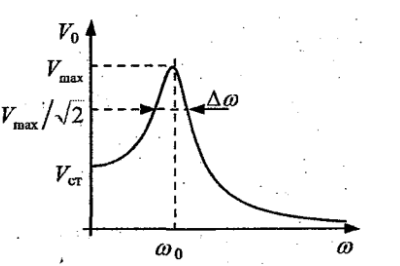
\includegraphics[scale = 0.9]{images/resonance.png}
        \caption{Резонансная кривая}
        \label{resonance}
    \end{figure}

    Нетрудно показать, что

    \begin{equation}
        \frac{U_{max}}{U_\text{ст}} = \frac{\omega_0}{2 \gamma}, \: Q = \frac{\omega_0}{2 \gamma} = \frac{\omega_0}{\Delta \omega}.
    \end{equation}

    \subsection{Процесс установления вынужденных колебаний}

    Рассмотрим процесс установления вынужденных колебаний. Для начала рассмотрим контур без затухания. После замыкания ключа в момент времени $t = 0$ в контуре благодаря ЭДС появляется ток. Уравнение для напряжения на конденсаторе имеет вид

    \begin{equation}
        \Dot{U} + \omega_0^2 U = \omega_0^2 \mathcal{E}_0 \cos \omega t.
    \end{equation}

    Решение этого уравнения запишем в виде суммы двух слагаемых, отвечающих соответственно свободным и вынужденным колебаниям

    \begin{equation}
        U(t) = a \cos{\omega_0 t} + b \sin{\omega_0 t} + \frac{\omega_0^2 \mathcal{E}_0}{\omega_0^2 - \omega^2} \cos{\omega t}.
    \end{equation}

    Из начальных условий $U(0) = 0$ и $\Dot{U}(0) = 0$, находим константы $a$ и $b$, в итоге получим

    \begin{equation}
        U(t) = \frac{\omega_0^2 \mathcal{E}_0}{\omega_0^2 - \omega^2} (\cos{\omega t} - \cos{\omega_0 t}) = \frac{-2 \omega_0^2 \mathcal{E}_0}{\omega_0^2 - \omega^2} \sin{(\frac{\omega - \omega_0}{2})} \sin{(\frac{\omega + \omega_0}{2})} 
    \end{equation}

    Найденное решение представляет собой быстро меняющийся гармонический сигнал (рис. \ref{pulse}), амплитуда которого медленно меняется по гармоническому закону. Такие колебания называются \textit{биениями}.

    \begin{figure}[H]
        \centering
        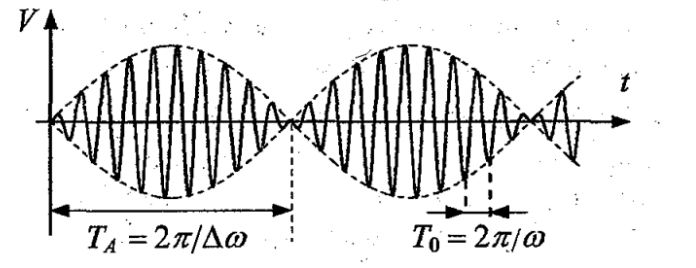
\includegraphics[scale = 0.5]{images/pulse.png}
        \caption{Биения до установления колебаний}
        \label{pulse}
    \end{figure}

    Если коэффициент затухания ненулевой, то свободные колебания со временем затухнут, и в контуре установятся гармонические вынужденные колебания (рис. \ref{ho}).

    \begin{figure}[H]
        \centering
        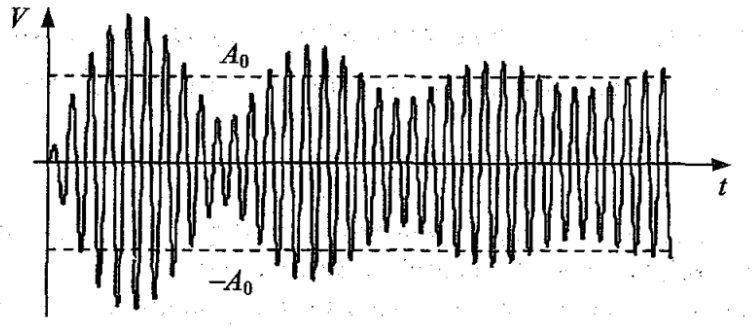
\includegraphics[scale = 0.5]{images/harmosc.png}
        \caption{Биения при установлении колебаний}
        \label{ho}
    \end{figure}

    Если на разряженный контур начать подавать внешнее напряжение с резонансной частотой, то амплитуда колебаний будет меняться по закону

    \begin{equation}
        U(t) = U_\infty \left( 1-e^{-\gamma t} \right).
    \end{equation}

    Аналогично, если выключить внешнее напряжение, то останутся только затухающие колебания, и амплитуда будет меняться по закону

    \begin{equation}
        U(t) = U_0 e^{-\gamma t}.
    \end{equation}

    \begin{figure}[H]
        \centering
        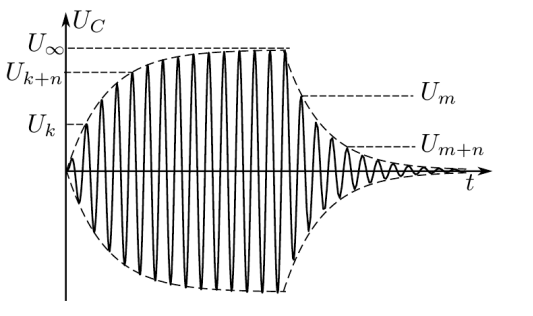
\includegraphics[scale = 0.7]{images/fosc.png}
        \caption{Нарастание и затухание вынужденных колебаний}
        \label{fosc}
    \end{figure}

    Таким образом, измеряя зависимость амплитуды от времени можно получить добротность $Q$:

    \begin{equation}
        Q = \pi \left( \frac{1}{n} \ln{\frac{U_\infty - U_k}{U_\infty - U_{k+n}}} \right)^{-1}.
    \end{equation}
    
    \section{Методика измерений и используемое оборудование}

    Схема установки для исследования колебаний приведена на рисунке \ref{installation}. Колебательный контур состоит из постоянной индуктивности $L$ с активным сопротивлением $R_L$, переменной емкости $С$ и сопротивления $R$. Картина колебаний напряжения на ёмкости наблюдается на экране двухканального осциллографа. Для возбуждения затухающих колебаний используется генератор сигналов специальной формы. Сигнал с генератора поступает через конденсатор $C_1$ на вход колебательного контура. Данная емкость необходима чтобы выходной импеданс генератора был много меньше импеданса колебательного контура и не влиял на процессы, проходящие в контуре.


    \begin{figure}[H]
        \centering
        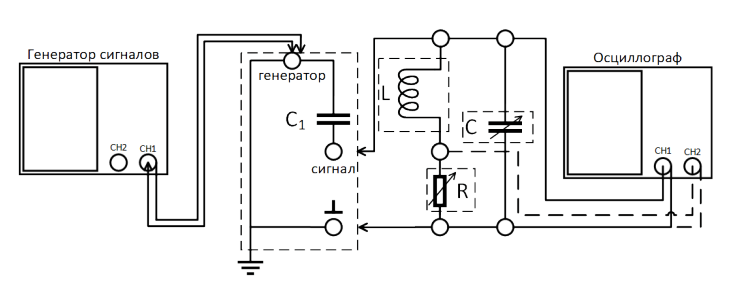
\includegraphics[scale = 0.8]{images/installation.png}
        \caption{ Схема установки для исследования вынужденных колебаний}
        \label{installation}
    \end{figure}
    
    Установка предназначена для исследования не только возбужденных, но и свободных колебаний в электрической цепи. При изучении свободно затухающих колебаний генератор специальных сигналов на вход колебательного контура подает периодические короткие импульсы, которые заряжают конденсатор $С$. За время между последовательными импульсами происходит разрядка конденсатора через резистор и катушку индуктивности. Напряжение на конденсаторе $U_c$ поступает на вход канала $1(X)$ электронного осциллографа. Для наблюдения фазовой картины затухающих колебаний на канал $2(Y)$ подается напряжение с резистора $R$ (пунктирная линия на схеме установки), которое пропорционально току $I$.
    
    При изучении возбужденных колебаний на вход колебательного контура подается синусоидальный сигнал. С помощью осциллографа возможно измерить зависимость амплитуды возбужденных колебаний в зависимости от частоты внешнего сигнала, из которого возможно определить добротность колебательного контура. Альтернативным способом расчета добротности контура является определение декремента затухания по картине установления возбуждённых колебаний. В этом случае генератор сигналов используется для подачи цугов синусоидальной формы.

    \section{Результаты измерений и обработка данных}

    \subsection{Измерение периода свободных колебаний}

    Для проведения эксперимента установили на магазине сопротивлений величину $R = 0$ Ом, на магазине индуктивностей $L = 100$ мГн, на магазине емкостей величину $С = 0$ мкФ. Несмотря на то, что на курбелях магазина емкостей стоит нулевое значение, контур сам по себе обладает некоторым минимальным значением ёмкости $C_0 = \frac{T}{4 \pi^2 L} = 0.001$ мкФ, благодаря которому в контуре реализуются свободные колебания. При этом затухание обеспечивалось наличием активного сопротивления в магазине индуктивностей $R_L$. Изменяя ёмкость (по курбелям), были проведены измерения периодов (табл. \ref{table:2.2.5}).
  
    \begin{table}[H]
        \centering
        \begin{tabular}{|c|c|c|c|c|}
        \hline
        $C$, мкФ & $C_0$, мкФ & $C_\Sigma$, мкФ & $T_{exp}$, мкс & $T_{theor}$, мкс \\ \hline
        0,000 & \multirow{8}{*}{0,001} & 0,001 & 69 & 63 \\ \cline{1-1} \cline{3-5} 
        0,001 &  & 0,002 & 94 & 89 \\ \cline{1-1} \cline{3-5} 
        0,002 &  & 0,003 & 113 & 109 \\ \cline{1-1} \cline{3-5} 
        0,003 &  & 0,004 & 128 & 126 \\ \cline{1-1} \cline{3-5} 
        0,004 &  & 0,005 & 144 & 140 \\ \cline{1-1} \cline{3-5} 
        0,005 &  & 0,006 & 157 & 154 \\ \cline{1-1} \cline{3-5} 
        0,007 &  & 0,008 & 181 & 178 \\ \cline{1-1} \cline{3-5} 
        0,009 &  & 0,010 & 202 & 199 \\ \hline
        \end{tabular}
        \caption{Результаты измерений периода свободных колебаний}
        \label{table:2.2.5}
    \end{table}

    Формулы, которые использовались при расчётах:

    \begin{equation}
        C_\Sigma = C_0 + C
    \end{equation}

    \begin{equation}
        T_{theor} = 2 \pi \sqrt{LC_\Sigma}
    \end{equation}


    По результатам измерений периода свободных колебаний, был построен график зависимости $T_{exp} = f (T_{theor})$. График изображён на рис. \ref{graph:exp(theor)}.

    \begin{figure}[H]
        \centering
        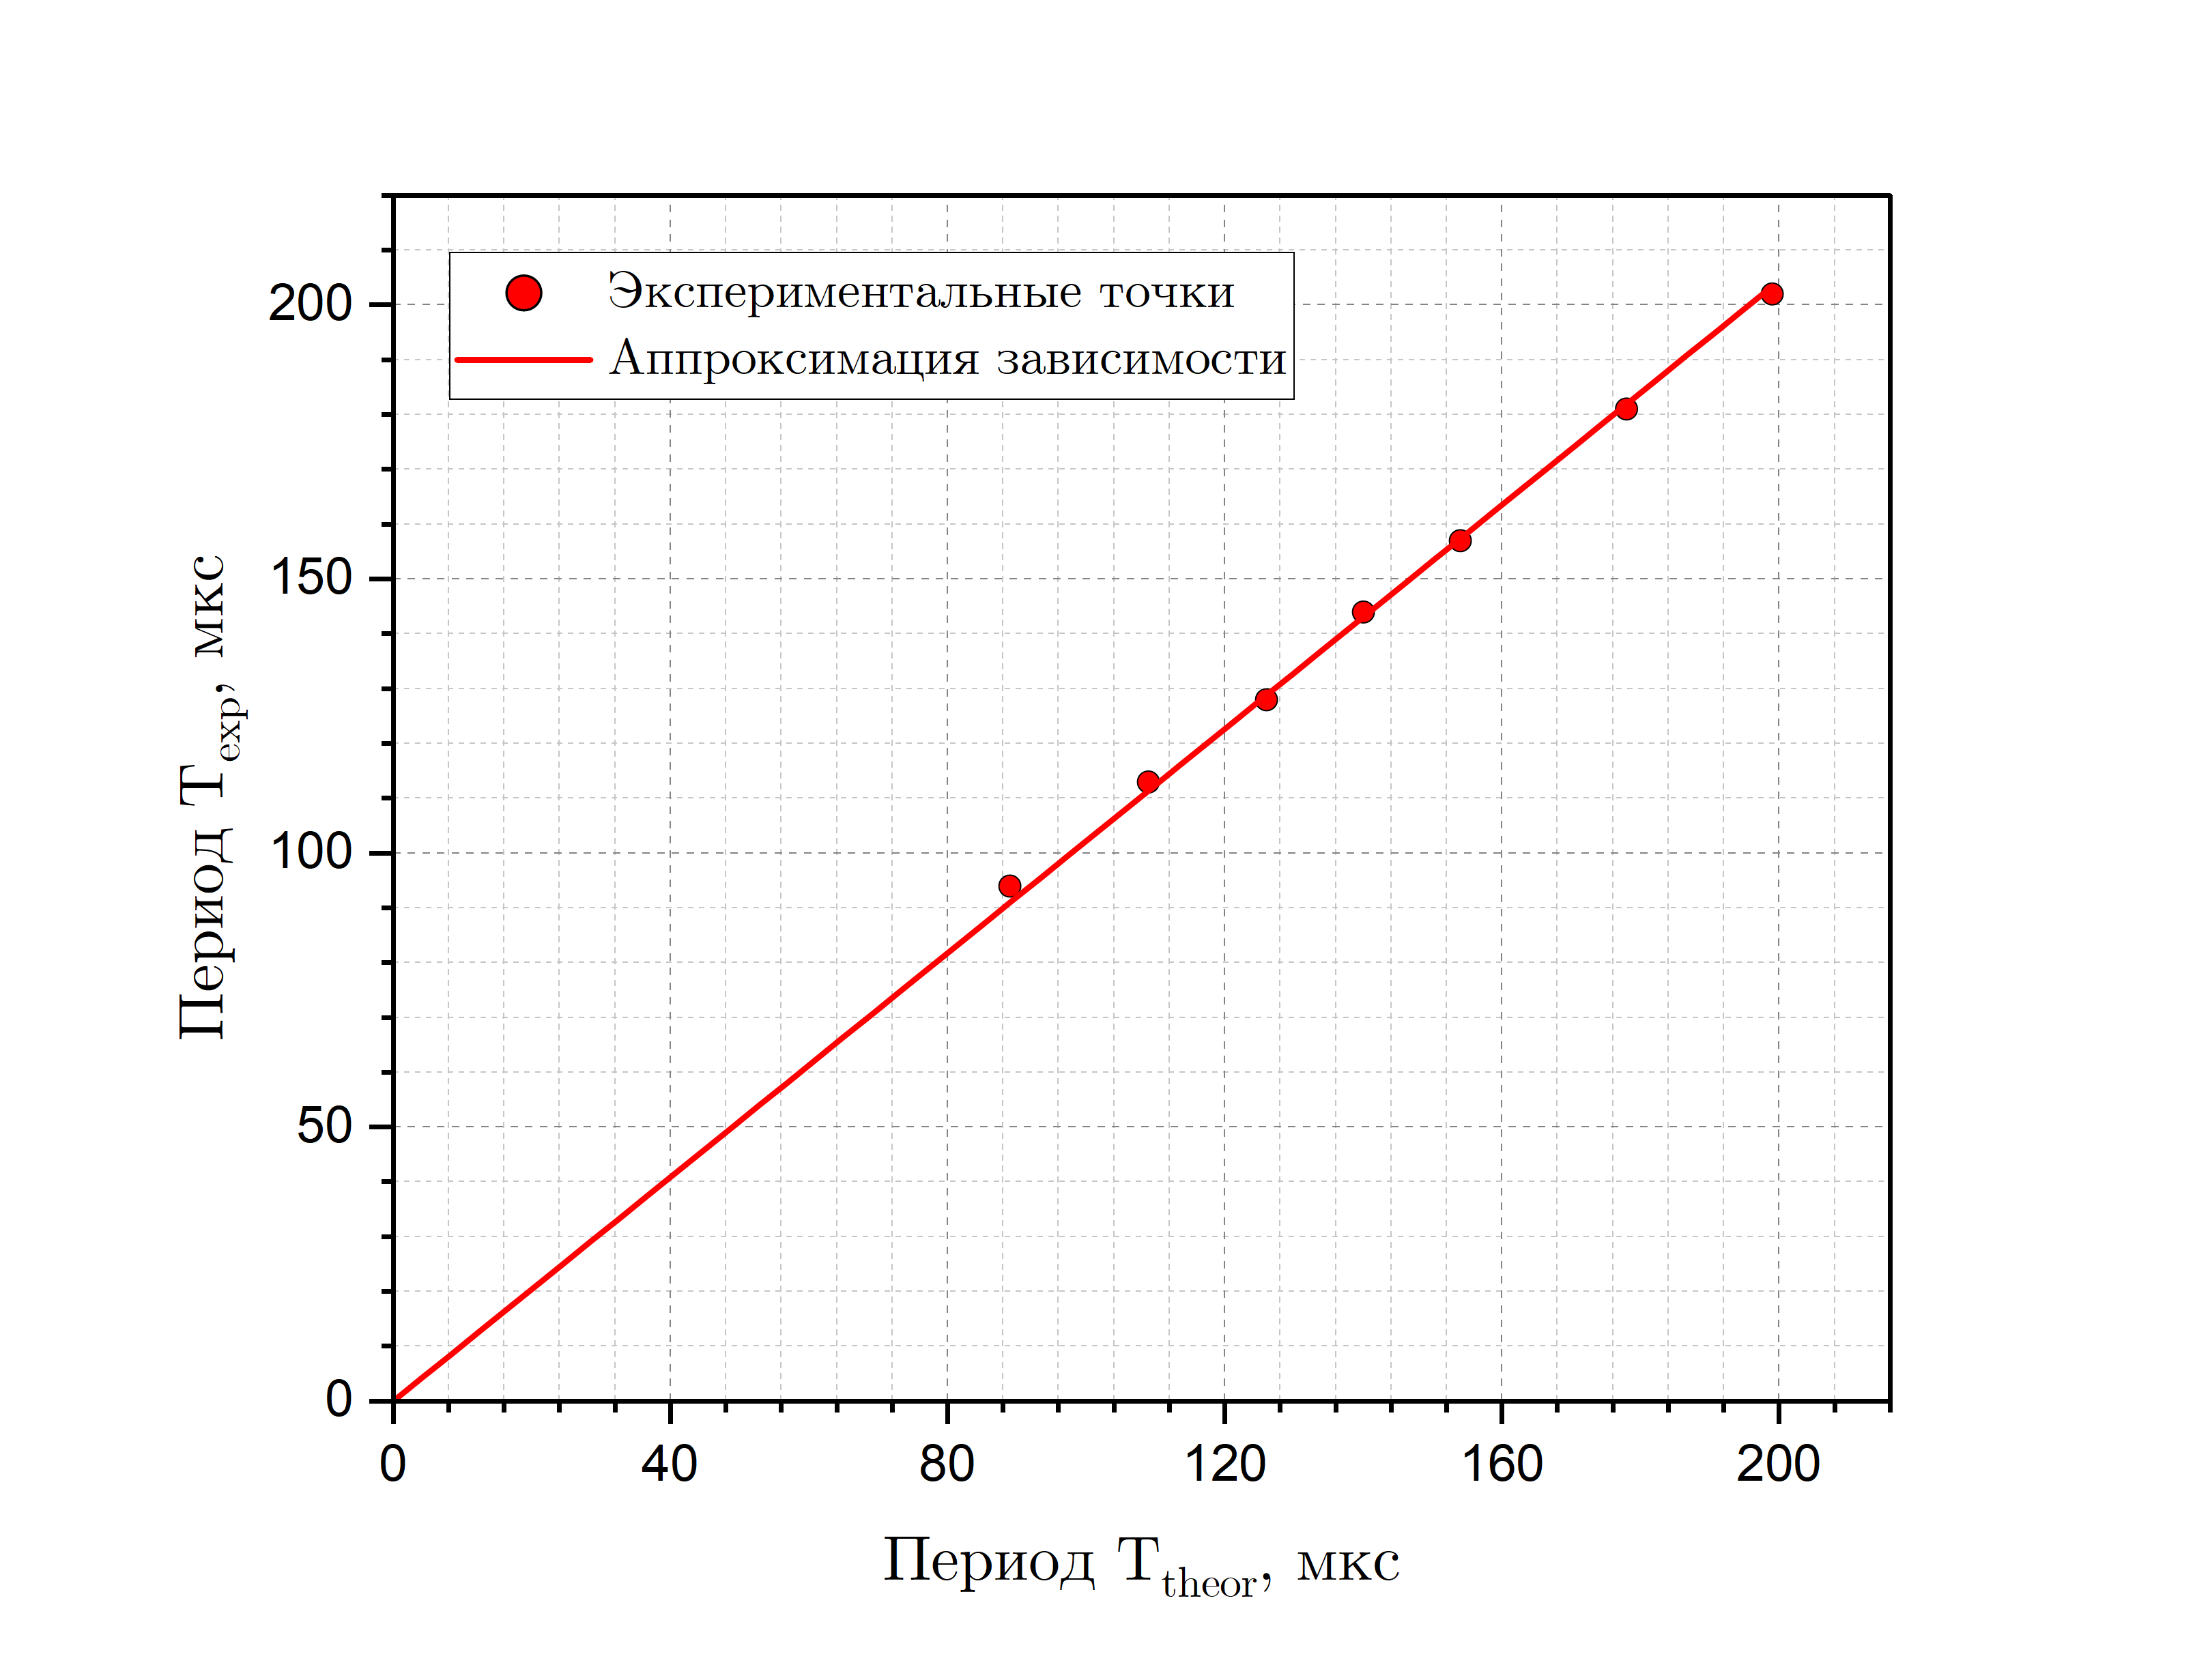
\includegraphics[scale = 0.6]{images/graph_exp(theor).png}
        \caption{График зависимости $T_{exp}$ от $T_{theor}$}
        \label{graph:exp(theor)}
    \end{figure}

    Аппроксимируя полученную зависимость в программе \textit{Origin Pro 2023}, получим коэффициент угла наклона:

    $$
    \boxed{k = \left( 1.006 \pm 0.004 \right)}
    $$

    Вследствие того, что $k \approx 1$ с учётом погрешности можно сказать, что изложенная теория находится в согласии с экспериментом.

    \subsection{Измерение логарифмического декремента затухания и критического сопротивления}

    Приняв $L = 100$ мГн, была рассчитана ёмкость $C^* = 6$ нФ, при которой собственная частота колебаний $\nu_0 = \frac{1}{2 \pi \sqrt{LC}} = 6.5$ кГц, и критическое сопротивление контура $R_{cr} = 2 \sqrt{\frac{L}{C^*}} = 8165$ Ом.

    Установив на магазине ёмкость, равную $C^* = 6$ нФ, и сопротивление $R \approx 0.05 R_{cr} \approx 408$ Ом, получили на экране осциллографа картину затухающих колебаний. Измеряя амплитуды колебаний, разделенных целым числом периодов $n$, были найдены логарифмические декременты затуханий $\Theta = \frac{1}{n} \ln{\frac{U_m}{U_{m+n}}}$ для различных значений $R$:

    $$
    \Theta_{0.05 R_{cr}} = \frac{1}{2} \ln{\frac{6.28}{3.12}} = 0.35
    $$

    $$
    \Theta_{0.08 R_{cr}} = \frac{1}{2} \ln{\frac{5.52}{1.72}} = 0.58
    $$

    $$
    \Theta_{0.11 R_{cr}} = \frac{1}{2} \ln{\frac{6.68}{1.42}} = 0.77
    $$

    $$
    \Theta_{0.14 R_{cr}} = \frac{1}{2} \ln{\frac{6.32}{0.90}} = 0.97
    $$

    $$
    \Theta_{0.17 R_{cr}} = \frac{1}{2} \ln{\frac{6.04}{0.59}} = 1.16
    $$

    $$
    \Theta_{0.20 R_{cr}} = \frac{1}{2} \ln{\frac{5.92}{0.37}} = 1.39
    $$

    Полученные данные представлены в таблице \ref{table:2.3.5}.
    
    \begin{table}[H]
        \centering
        \begin{tabular}{|c|c|c|c|}
        \hline
        $R$, Ом & $\Theta$ & $1/R^2, 10^{-6} \cdot \text{ Ом}^{-2}$ & $1/\Theta^2$ \\ \hline
        408 & 0,35 & 6,00 & 8,16 \\ \hline
        653 & 0,58 & 2,34 & 2,97 \\ \hline
        898 & 0,77 & 1,24 & 1,69 \\ \hline
        1143 & 0,97 & 0,77 & 1,06 \\ \hline
        1388 & 1,16 & 0,52 & 0,74 \\ \hline
        1633 & 1,39 & 0,37 & 0,52 \\ \hline
        \end{tabular}
        \caption{Результаты измерения зависимости $1/\Theta^2 = f(1/R^2)$}
        \label{table:2.3.5}
    \end{table}

    По таблице \ref{table:2.3.5} был построен график зависимости $1/\Theta^2$ от $1/R^2$ (рис. \ref{graph:theta}).

    \begin{figure}[H]
        \centering
        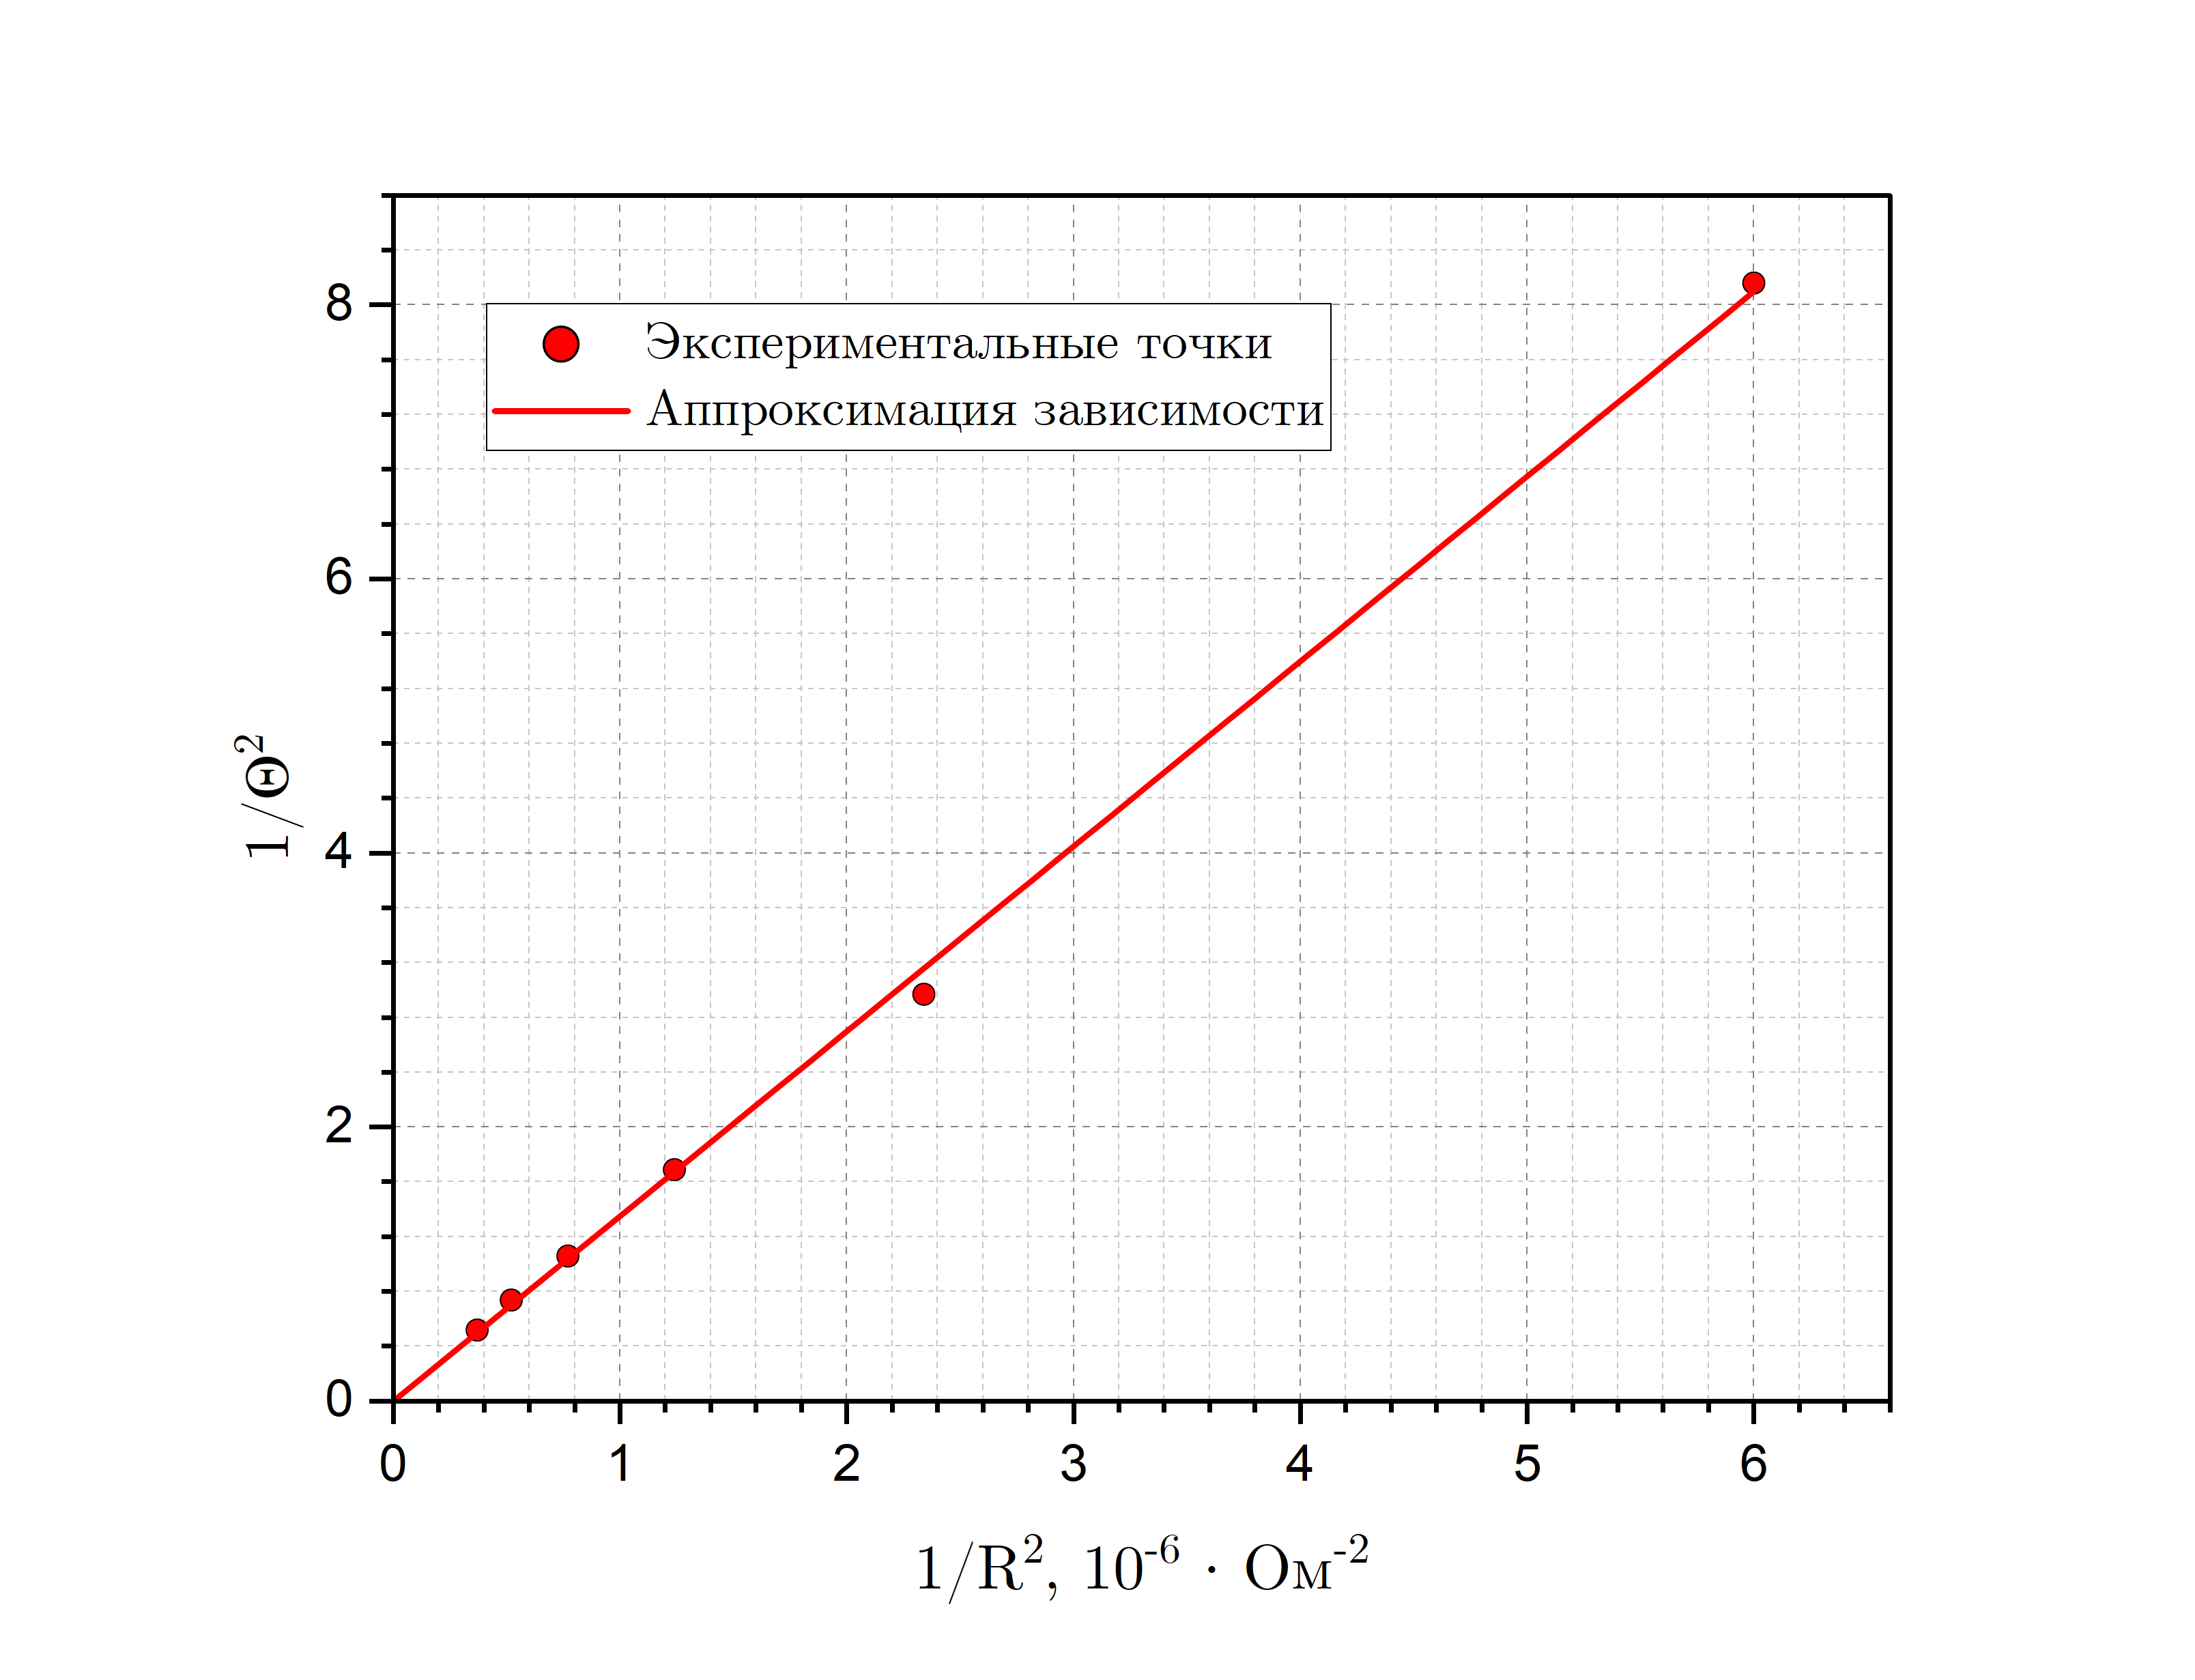
\includegraphics[scale = 0.6]{images/graph_theta.png}
        \caption{График зависимости $1/\Theta^2$ от $1/R^2$}
        \label{graph:theta}
    \end{figure}

     Аппроксимируя полученную зависимость в программе \textit{Origin Pro 2023}, получим коэффициент угла наклона:

     $$
     \frac{\Delta Y}{\Delta X} = \left( 1.35 \pm 0.01 \right) \cdot 10^6 \cdot \text{Ом}^2,
     $$

     где $Y = 1/\Theta^2$, а $X = 1/R^2$. Отсюда, можно вычислить $R_{cr} = 2 \pi \sqrt{\Delta Y / \Delta X} = 7300$ Ом и $\Delta R_{cr} = 30$ Ом.

     Окончательно получим:

     $$
     \boxed{R_{cr} = \left( 7300 \pm 30 \right) \text{ Ом}}
     $$

     Заметим, что экспериментальное значение $R_{cr}$ немного отличается от теоретического. Это можно объяснить тем, что в работе не учитывалось сопротивление остальной части цепи.

     \subsection{Измерение добротности контура}

    В начале определим добротность контура $Q = \pi / \Theta$, воспользовавшись результатами предыдущего пункта. Полученные значения приведены в таблице \ref{table:Q_1}.

    \begin{table}[H]
        \centering
        \begin{tabular}{|c|c|c|c|c|c|c|}
        \hline
        $R$, Ом & 408 & 653 & 898 & 1143 & 1388 & 1633 \\ \hline
        $\Theta$ & 0,35 & 0,58 & 0,77 & 0,97 & 1,16 & 1,39 \\ \hline
        $Q$ & 8,98 & 5,42 & 4,08 & 3,24 & 2,71 & 2,26 \\ \hline
        \end{tabular}
        \caption{Результаты вычисления добротности первым способом}
        \label{table:Q_1}
    \end{table}

    Теперь определим добротность контура другим способом, наблюдая затухающие колебания на фазовой плоскости. Для определения декремента затухания измерим координаты пересечения витков спирали с одной из осью координат (рис. \ref{osc}), разделенные целым числом периодов $n$. Полученные значения приведены в таблице \ref{table:Q_2}.

    \begin{figure}[H]
        \centering
        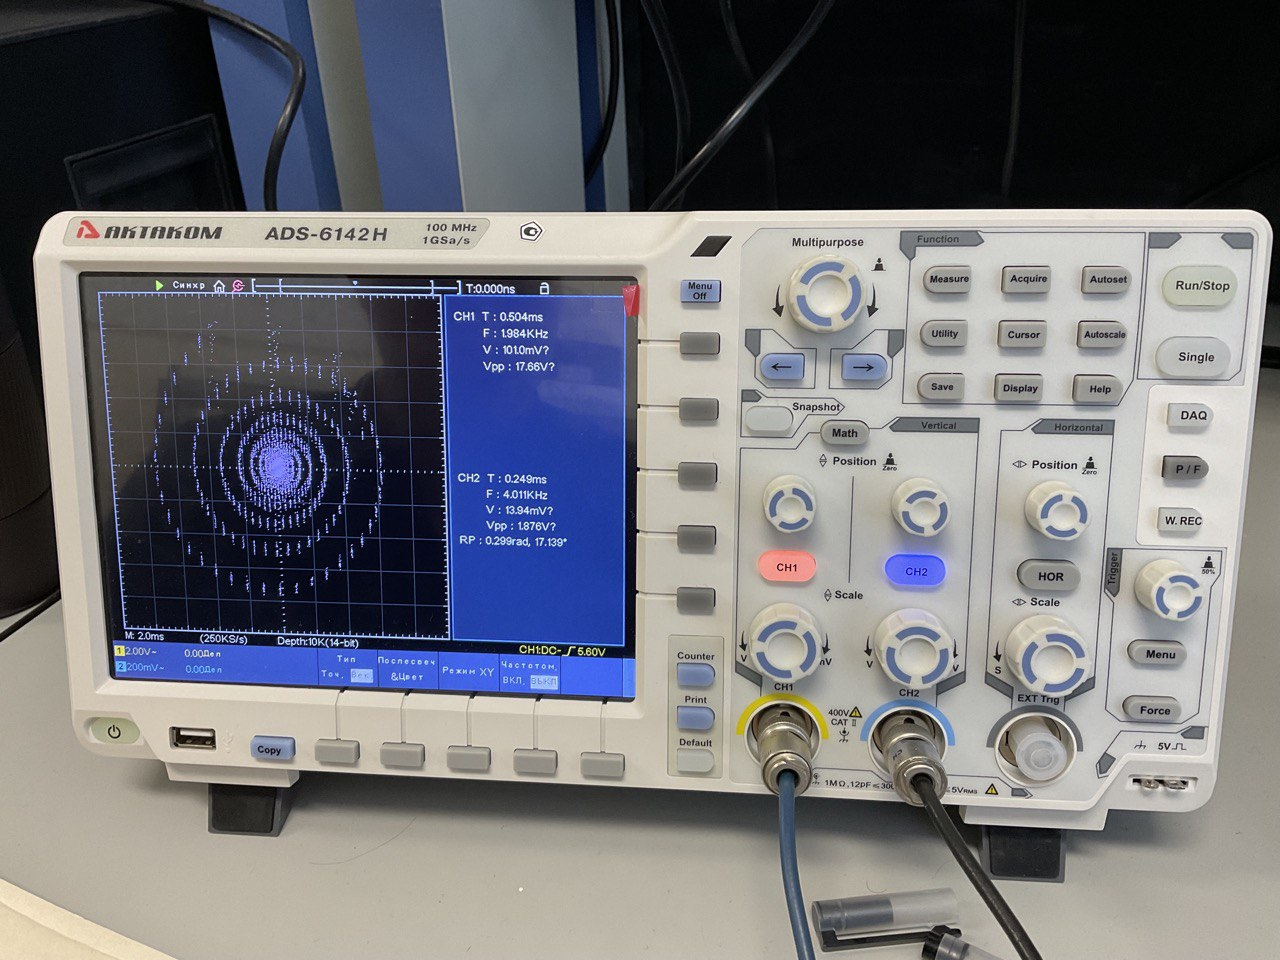
\includegraphics[scale = 0.3]{images/osc.jpg}
        \caption{Фазовая плоскость затухающих колебаний на осциллографе}
        \label{osc}
    \end{figure}

    \begin{table}[H]
        \centering
        \begin{tabular}{|c|c|c|c|c|c|c|}
        \hline
        $R$, Ом & 408 & 653 & 898 & 1143 & 1388 & 1633 \\ \hline
        $\Theta$ & 0,31 & 0,59 & 0,79 & 0,92 & 1,22 & 1,32 \\ \hline
        $Q$ & 10,13 & 5,33 & 3,98 & 3,43 & 2,57 & 2,38 \\ \hline
        \end{tabular}
        \caption{Результаты вычисления добротности вторым способом}
        \label{table:Q_2}
    \end{table}

    Наконец, рассчитаем теоретическое значение добротности через параметры контура $L = 100$ мГн, $C = 6$ нФ и $R$ по формуле $Q  = \frac{1}{R} \sqrt{\frac{L}{C}}$. Полученные значения приведены в таблице \ref{table:Q_3}.

     \begin{table}[H]
        \centering
        \begin{tabular}{|c|c|c|c|c|c|c|}
        \hline
        $R$, Ом & 408 & 653 & 898 & 1143 & 1388 & 1633 \\ \hline
        $Q$ & 10,00 & 6,25 & 4,55 & 3,57 & 2,94 & 2,50 \\ \hline
        \end{tabular}
        \caption{Результаты вычисления добротности вторым способом}
        \label{table:Q_3}
    \end{table}

    \section{Заключение}

    Результаты работы (измерения добротности контура различными способами) приведены в таблице \ref{table:final}.

    \begin{table}[H]
        \centering
        \begin{tabular}{|c|ccc|}
        \hline
        \multirow{2}{*}{$R$, Ом} & \multicolumn{3}{c|}{Свободные колебания} \\ \cline{2-4} 
         & \multicolumn{1}{c|}{$f(L, C, R)$} & \multicolumn{1}{c|}{$f(\Theta)$} & Спираль \\ \hline
        408 & \multicolumn{1}{c|}{10,00} & \multicolumn{1}{c|}{8,98} & 10,13 \\ \hline
        653 & \multicolumn{1}{c|}{6,25} & \multicolumn{1}{c|}{5,42} & 5,33 \\ \hline
        898 & \multicolumn{1}{c|}{4,55} & \multicolumn{1}{c|}{4,08} & 3,98 \\ \hline
        1143 & \multicolumn{1}{c|}{3,57} & \multicolumn{1}{c|}{3,24} & 3,43 \\ \hline
        1388 & \multicolumn{1}{c|}{2,94} & \multicolumn{1}{c|}{2,71} & 2,57 \\ \hline
        1633 & \multicolumn{1}{c|}{2,50} & \multicolumn{1}{c|}{2,26} & 2,38 \\ \hline
        \end{tabular}
        \caption{Результаты лабораторной работы}
        \label{table:final}
    \end{table}

    Исходя из данных таблицы \ref{table:final} можно сказать, что значения, полученные всеми способами определения добротности колебательной системы, предложенными для проверки, согласуются с теоретическими значениями добротности в различных конфигурациях.

\end{document}